\documentclass[12pt]{article}

\usepackage{geometry}
\usepackage{amsmath,amsthm,amssymb}
\usepackage{graphicx}
\usepackage{multicol}

\newcommand{\lemma}{\noindent \textbf{Lemma: }}
\newcommand{\thm}{\noindent \textbf{Theorem: }}
\newcommand{\lskip}{\vspace{\baselineskip}}

\begin{document}

\title{Splay Trees}
\author{}
\maketitle

\section*{Description}
AVL trees are self-balancing BSTs that are not strictly balanced. On each access (query or insert), the accessed node is splayed up to the root of the tree. This results in faster runtimes times when nodes are repeatedly access. In this way, a splay tree functions as a cache.

\section*{Splaying}
There are four cases for splaying an accessed node $x$.
\begin{enumerate}
  \item $x$ is the root. In this case there is nothing to do.
  \item Zig/Zag: $x$ is the left/child child of the root.
    \begin{figure}[!ht]
      \centering
      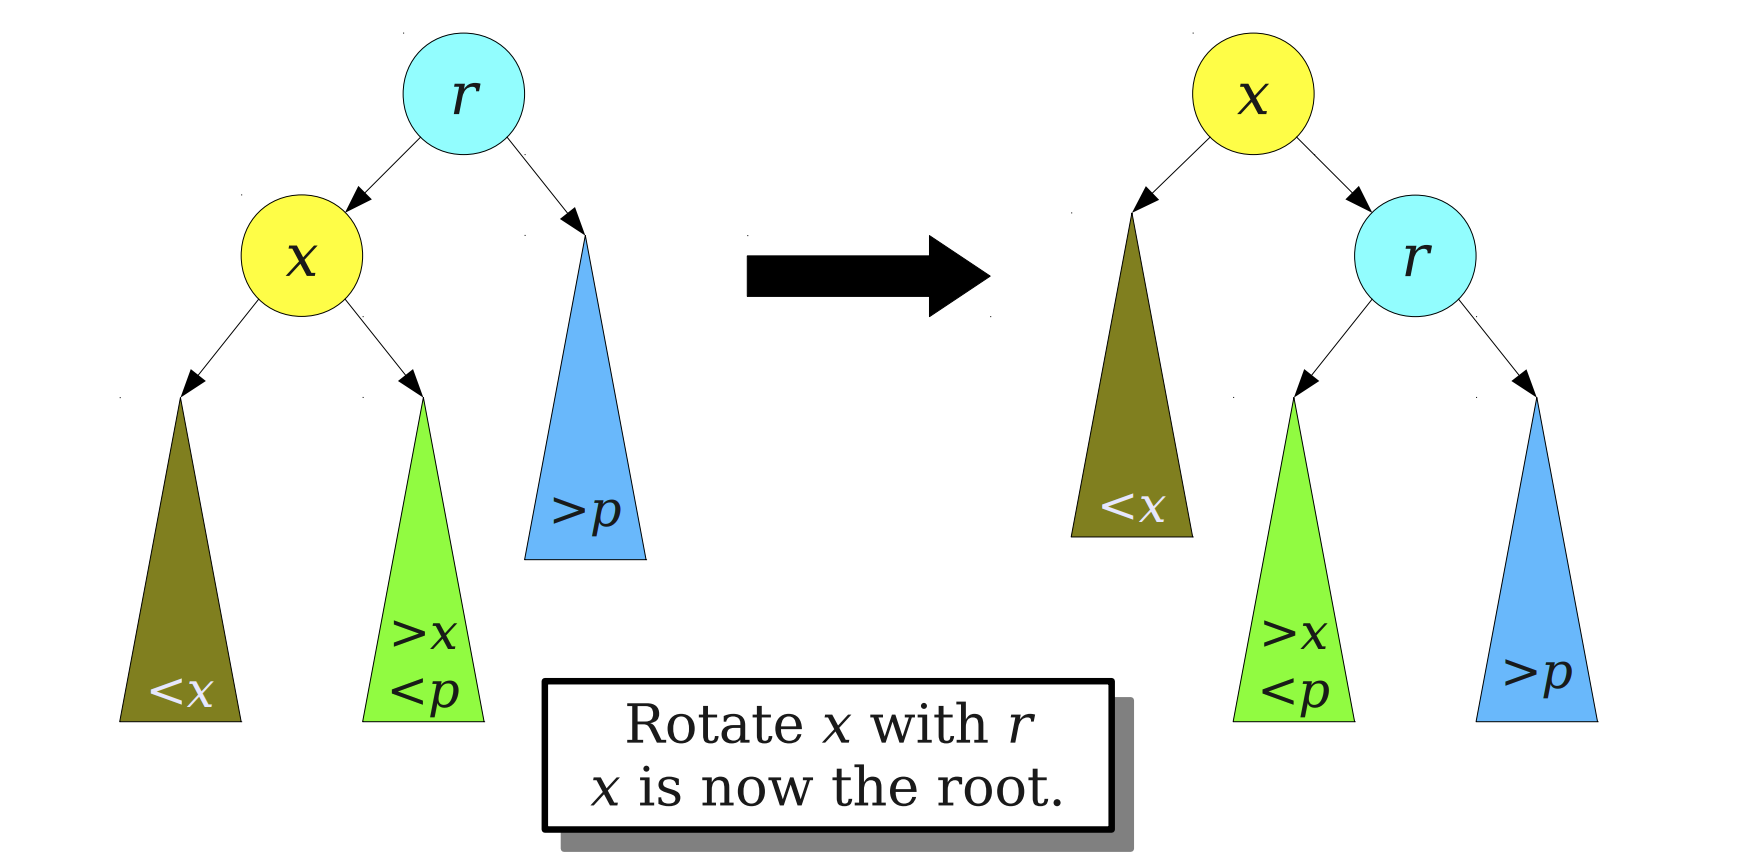
\includegraphics[scale=0.16]{pics/splay_zig}
      \caption{Zig Rotation}
    \end{figure}
  \item Zig-Zig/Zag-Zag: $x$ is the left/right child of $p$ and $p$ is the left/right child of $g$. \\
    \begin{figure}[!ht]
      \centering
      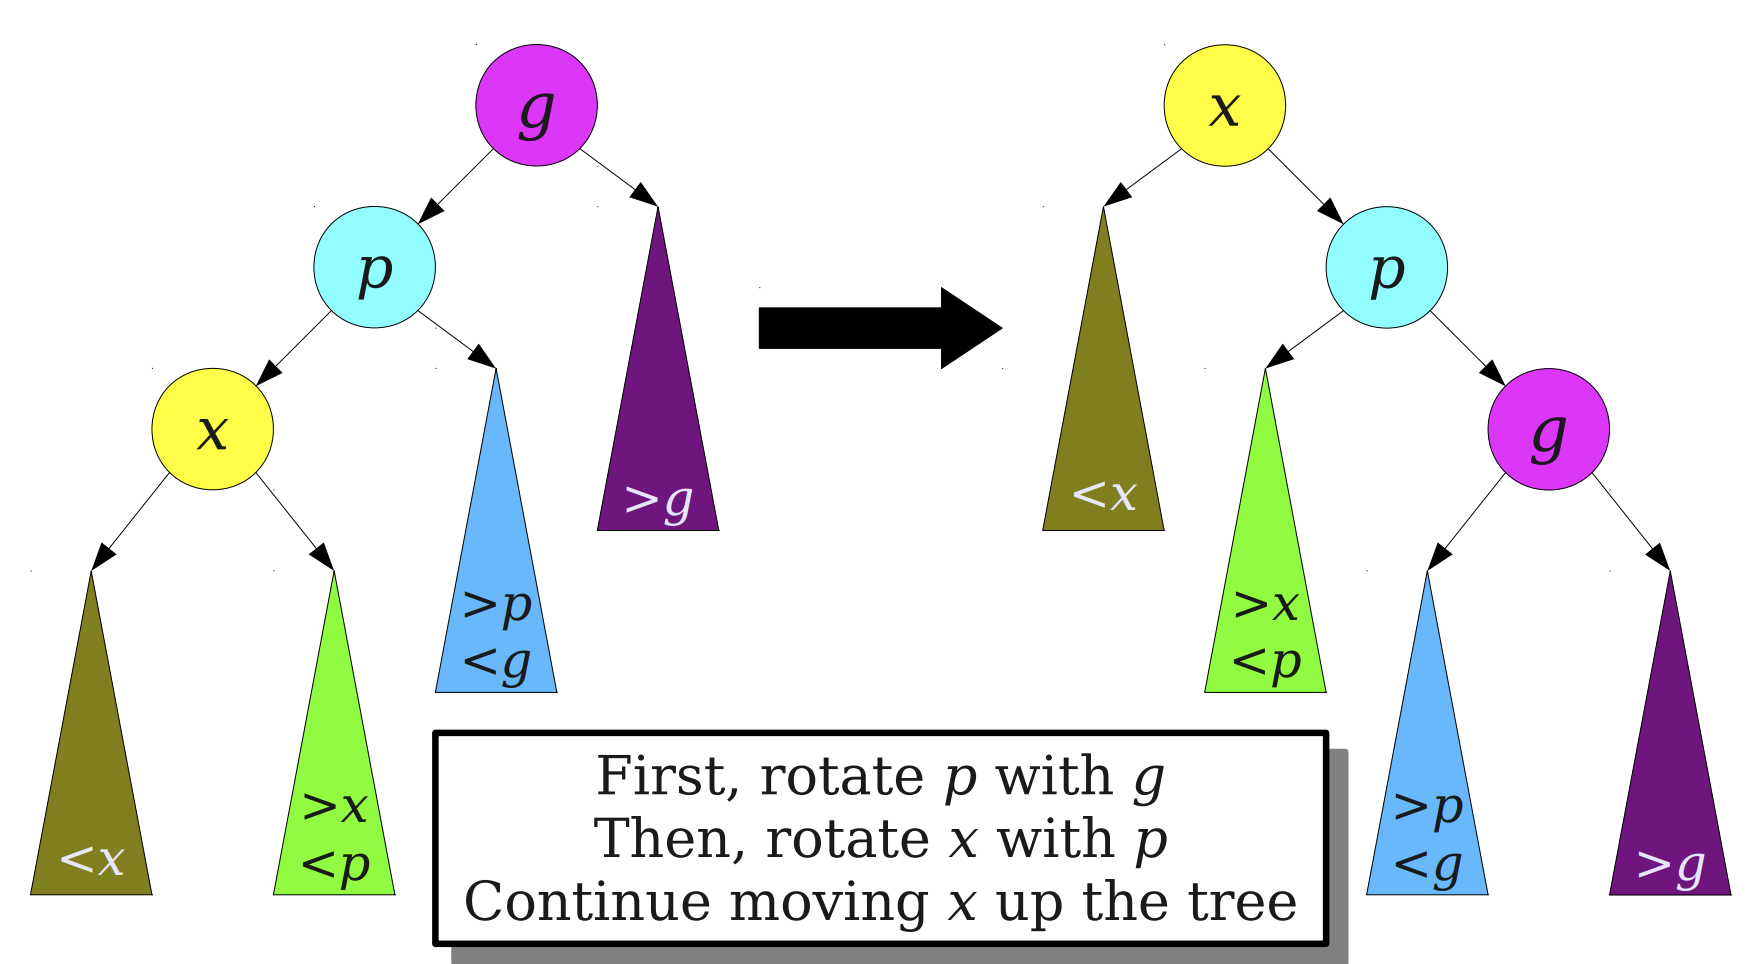
\includegraphics[scale=0.16]{pics/splay_zig_zig}
      \caption{Zig-Zig Rotation}
    \end{figure}
  \item Zig-Zag/Zag-Zig: $x$ is the left/right child of $p$ and $p$ is the right/left child of $g$. \\
    \begin{figure}[!ht]
      \centering
      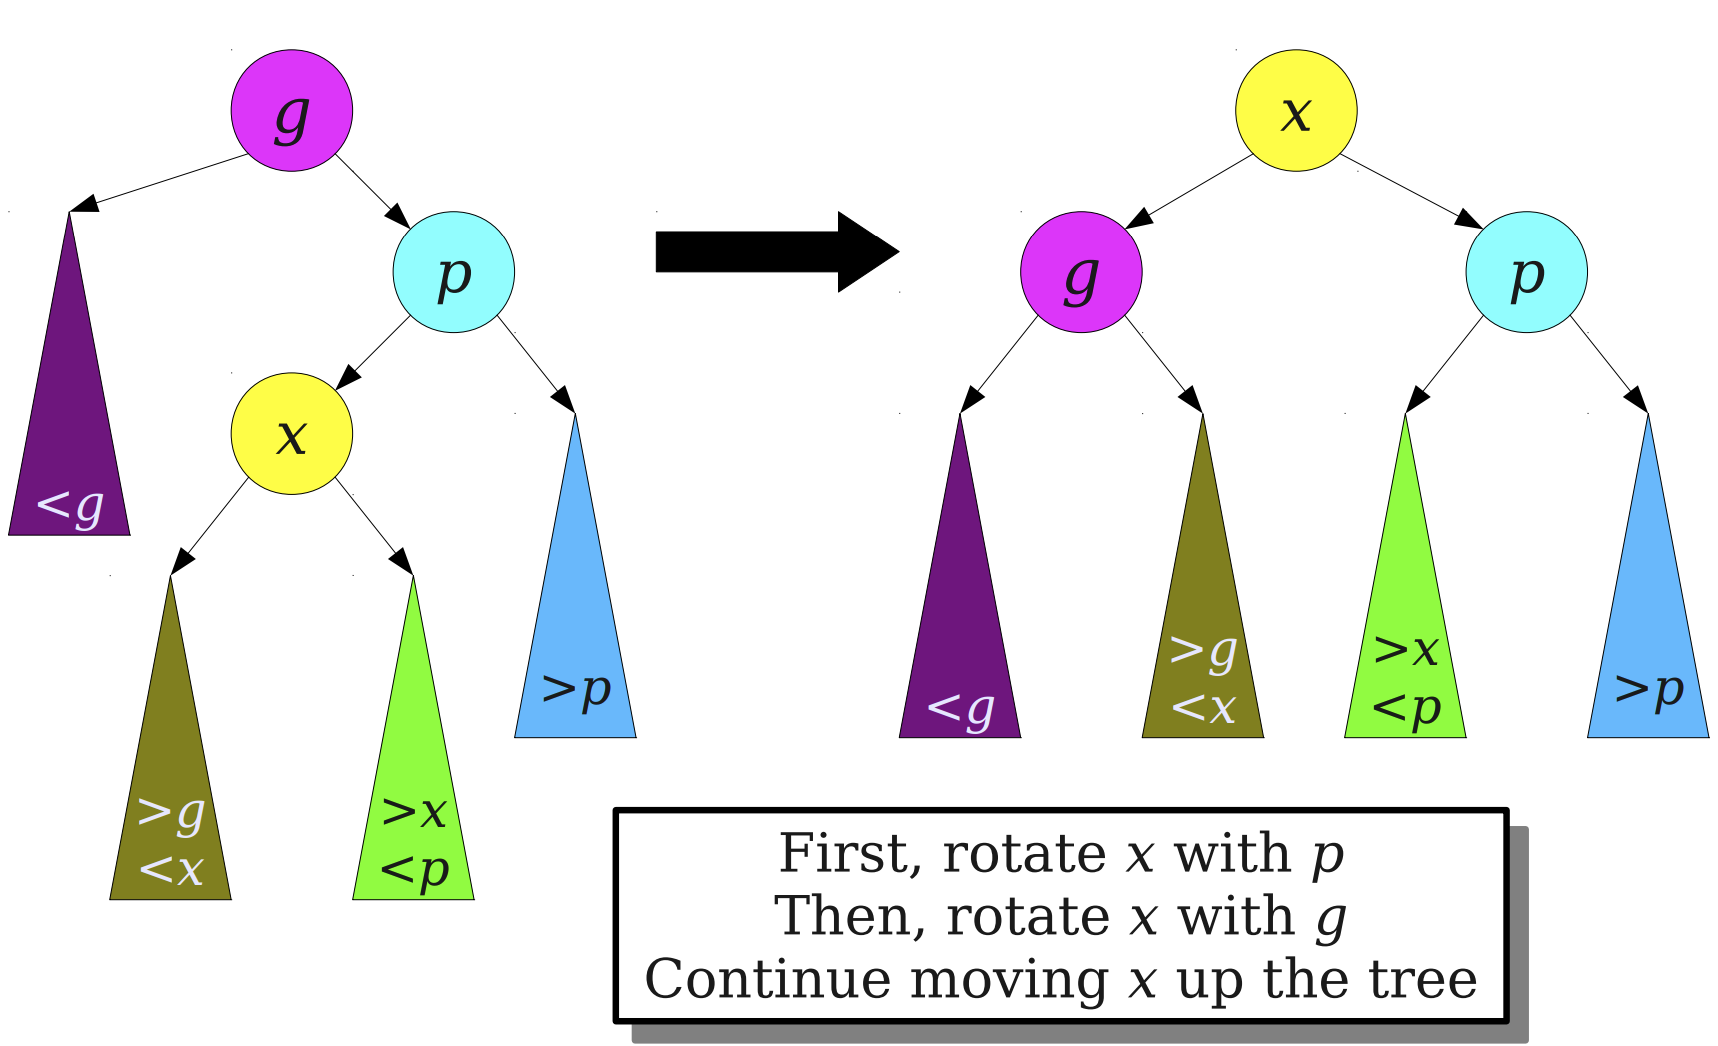
\includegraphics[scale=0.16]{pics/splay_zig_zag}
      \caption{Zag-Zig Rotation}
    \end{figure}
\end{enumerate}

\section*{Time Complexity}
We will analyze the time complexity of a splay using the potential method. We define the \emph{size} of a node $x_i$ to be the size of the subtree rooted at $x_i$. Next, define the \emph{rank} of a node $x$ to be $r(x) = \log s(x)$. Letting $n$ be the number of nodes in the tree, our potential function will be
\[ \Phi = \sum_{i=1}^n r(x_i) \]
We claim this satisfies the requirements of a potential function. First, $\Phi_1 = 0$. Since $s(x_i) \geq 1$, $r(x_i) \geq 0$, so $\Phi_i \geq 0 \ \forall i$.
\lskip

\begin{lemma}
  If $x>0, y>0$, and $x+y \leq 1$, then $\log x + \log y \leq -2$.
\end{lemma}

\begin{proof}
  First, $\log x + \log y = \log (xy)$. Since $\log$ is strictly increasing, we can equivalently maximize $xy$. Since $x$ and $y$ are nonnegative, the maximum value of $xy$ will clearly occur when $x+y=1$.

  Then $y = x-1$, so we are maximizing $x(1-x)$. Setting the derivative to 0 gives us
  \begin{align*}
    1-2x &= 0 \\
    x &= \frac{1}{2}
  \end{align*}
  Then $y = \frac{1}{2}$ and $\log x + \log y = -1 + -1 = -2$.
\end{proof}

We will now calculate the amortized cost of each rotation within a splay individually. Then, we will use these results to show that the amortized cost of splaying a node $x$ in a tree with root $t$ is at most $3(r(t) - r(x)) + 1$. In each of the following calculations, let $r'(x)$ denote the rank of $x$ after the rotation.

\begin{enumerate}
  \item $x$ is the root. $O(1)$.
  \item Zig/Zag:
  \begin{figure}[!ht]
    \centering
    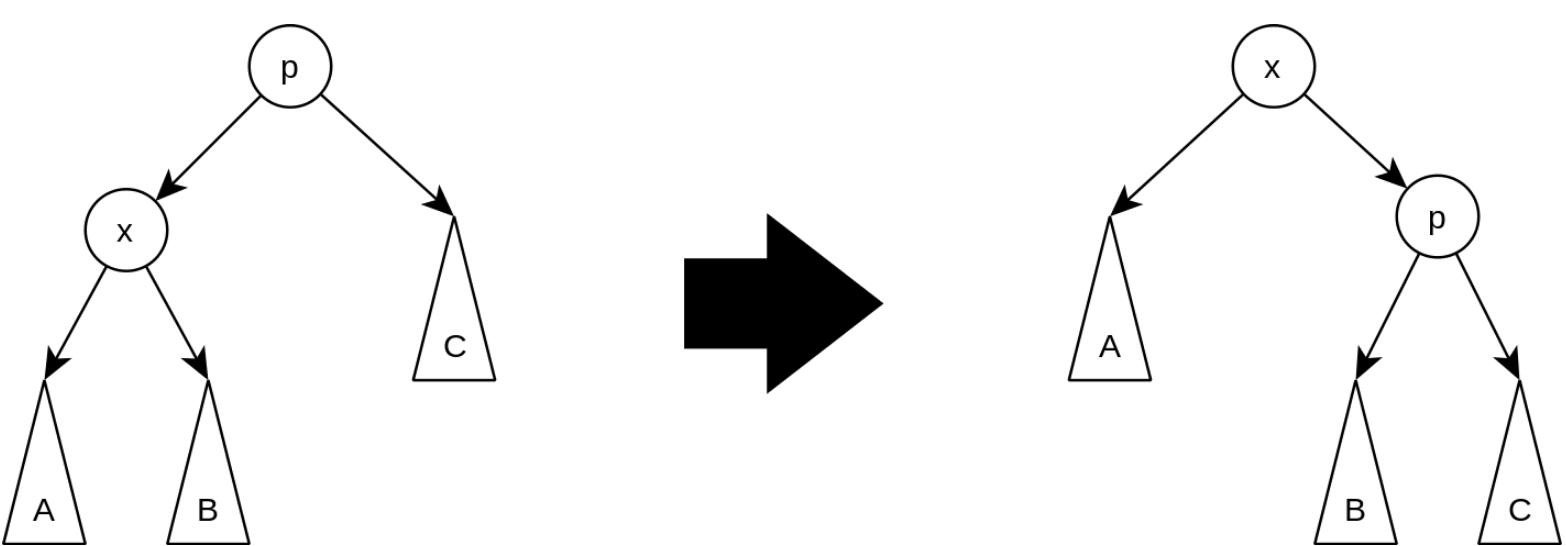
\includegraphics[scale=0.2]{pics/splay_zig2}
  \end{figure}

  The actual cost of operation is 1, since a single rotation is required. We now claim that the change in potential is at most $3(r'(x) - r(x))$, or equivalently, that $\Delta\Phi - 3r'(x) + 3r(x) \leq 0$. To that end, we can see from the figure that
  \[ \Delta\Phi = r'(x) + r'(p) - r(x) - r(p) \]
  Now we have
  \begin{align*}
    \Delta\Phi - 3r'(x) + 3r(x) &= r'(x) + r'(p) - r(x) - r(p) - 3r'(x) + 3r(x) \\
    &= r'(p) - r(p) - 2r'(x) + 2r(x) \\
    &\leq r'(x) - r(p) - 2r'(x) + 2r(x) \\
    &\leq r'(x) - r(x) - 2r'(x) + 2r(x) \\
    &= -r'(x) + r(x) \\
    &= \log s(x) - \log s'(x) \\
    &= \log \frac{s(x)}{s'(x)}
  \end{align*}
  Since $s(x) \leq s'(x)$, $\frac{s(x)}{s'(x)} \leq 1$, and thus $\log \frac{s(x)}{s'(x)} \leq 0$. Altogether, amortized cost of a Zig (actual cost plus the change in potential) is at most
  \[ 1 + 3(r'(x) - r(x)) \]

  \item Zig-Zig/Zag-Zag:
  \begin{figure}[!ht]
    \centering
    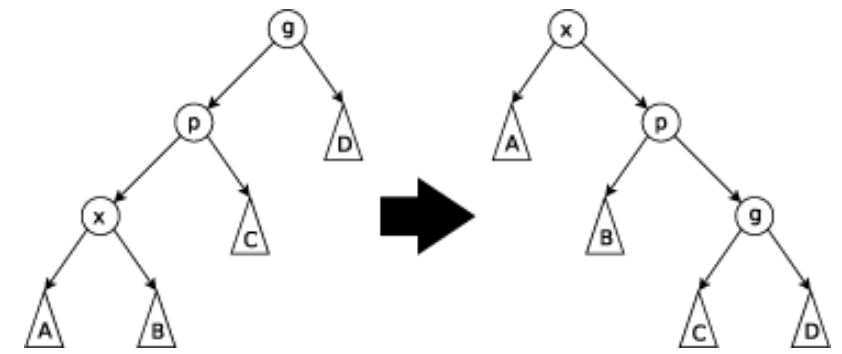
\includegraphics[scale=0.33]{pics/splay_zig_zig2}
  \end{figure}
  The actual cost of the operation is 2, since two rotations are required. We now claim that the change in potential is at most $3(r'(x) - r(x)) - 2$, or equivalently, that $\Delta\Phi -3r'(x) + 3r(x) \leq -2$. To that end, we can see from the figure that
  \[ \Delta\Phi = r'(x) + r'(p)+ r'(g) - r(x) - r(p) - r(g) \]
  We can also see that $r(g) = r'(x)$, so these cancel, giving us
  \[ \Delta\Phi = r'(p)+ r'(g) - r(x) - r(p) \]
  Now, we have
  \begin{align*}
    \Delta\Phi -3r'(x) + 3r(x) &= r'(p) + r'(g) - r(x) - r(p) -3r'(x) + 3r(x) \\
    &= r'(p) + r'(g) - r(p) - 3r'(x) + 2r(x)\\
    &\leq r'(x) + r'(g) - r(p) - 3r'(x) + 2r(x)\\
    &\leq r'(g) + r'(g) - r(x) - 3r'(x) + 2r(x)\\
    &= r'(g) - 2r'(x) + r(x)\\
    &= r(x) - r'(x) + r'(g) - r'(x)\\
    &= \log s(x) - \log s'(x) + \log s'(g) - \log s'(x)\\
    &= \log \frac{s(x)}{s'(x)} + \log \frac{s'(g)}{s'(x)} \\
  \end{align*}
  Clearly $\frac{s(x)}{s'(x)}, \frac{s'(g)}{s'(x)} > 0$, but we also need to show that $\frac{s(x)}{s'(x)} + \frac{s'(g)}{s'(x)} \leq 1$ to use our lemma. Equivalently, we'll show that $s(x) + s'(g) \leq s'(x)$. We can see that
  \begin{align*}
    s(x) &= w(x) + s(A) + s(B) \\
    s'(g) &= w(g) + s(C) + s(D) \\
    s'(x) &= w(x) + w(p) + w(g) + s(A) + s(B) + s(C) + s(D) \\
  \end{align*}
  so $s(x) + s'(g) \leq s'(x)$. Therefore, we can apply our lemma to get
  \[ \log \frac{s(x)}{s'(x)} + \log \frac{s'(g)}{s'(x)} \leq -2 \]
  Altogether, amortized cost of a Zig-Zig is at most
  \[ 2 + 3(r'(x) - r(x)) - 2 = 3(r'(x) - r(x)) \]

  \item Zig-Zag/Zag-Zig:
  \begin{figure}[!ht]
    \centering
    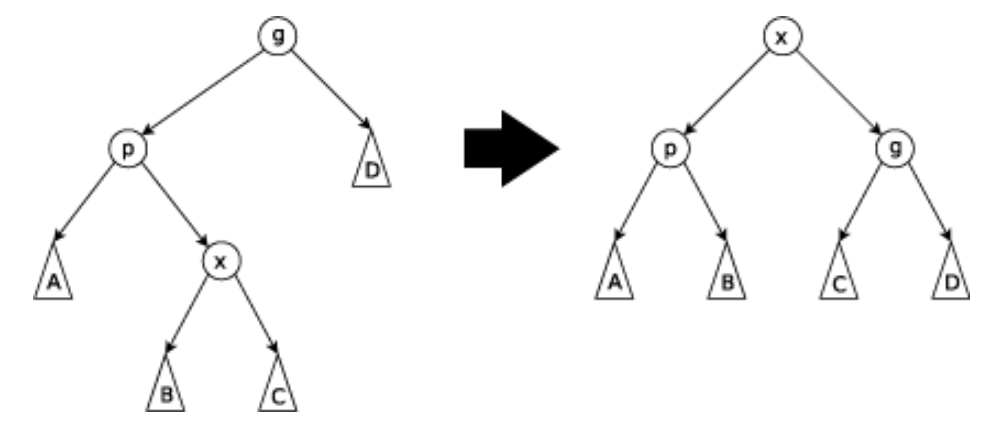
\includegraphics[scale=0.33]{pics/splay_zig_zag2}
  \end{figure}

  Again, the actual cost is 2 and we will show that $\Delta\Phi - 3r'(x) + 3r(x) \leq -2$. To that end
  \[ \Delta\Phi = r'(x) + r'(p)+ r'(g) - r(x) - r(p) - r(g) \]
  Since $r(g) = r'(x)$, we have
  \begin{align*}
    \Delta\Phi - 3r'(x) + 3r(x) &= r'(p) + r'(g) - r(x) - r(g) - 3r'(x) + 3r(x) \\
    &= r'(p) + r'(g) - r(g) - 3r'(x) + 2r(x) \\
    &\leq r'(x) + r'(g) - r(x) - 3r'(x) + 2r(x) \\
    &= r'(g) - 2r'(x) + r(x) \\
  \end{align*}
  This is now the same as the previous case, so the amortized cost of a Zig-Zag is also at most
  \[ 2 + 3(r'(x) - r(x)) - 2 = 3(r'(x) - r(x)) \]
\end{enumerate}

Now, suppose the splay contains  $k$ Zig-Zig/Zig-Zag rotations. Via a telescoping argument, the total amortized cost of these rotations is
\[ 3(r'(x) - r(x)) + 3(r''(x) - r'(x)) + \ldots + 3(r^{(k)}(x) - r^{(k-1)}(x)) = 3(r^{(k)}(x) - r(x)) \]

Note that there can be at most one Zig/Zag operation, since it only occurs when the accessed node is a child of the root. This has an amortized cost of $3(r^{(k+1)}(x) - r^{(k)}(x)) + 1$. Because $x$ is at the root at the end of this splay, we know $r^{(k+1)}(x) = r(t)$, where $t$ is the original root of the tree. So, altogether we have an amortized cost of $3(r^{(k)}(x) - r(x)) + 3(r(t) - r^{(k)}(x)) + 1 = 3(r(t) - r(x)) + 1$.

Now, we note that $s(t) = n$, which means $r(t) = \log n$, and $s(x) \geq 1$, which means $r(x) \geq 0$. Therefore the amortized cost of a splay is at most
\[ 3(r(t) - r(x)) + 1 \leq 3(\log n - 0) + 1 \in O(\log n)\]
So, for $m$ operations, $T_{amortized}(m) = O(m \log n)$.
\end{document}
